\documentclass[french]{RMcv}
%
\hypersetup{%
  % Language related
  pdftitle={CV Milani},%
  pdfkeywords=CV,%
  pdflang=fr-FR,%
}

\renewcommand\intracvevent{4pt} % Spacing between a cvevent and the previous object. Default: 6pt
%\renewcommand\intercvevent{4pt} % Spacing between first line and bullet point of a cvevent. Default: 6pt

\title{CV - Fra}

\newif\ifcvtitle
\newif\ifcvsubtitle
\cvtitlefalse
\cvsubtitlefalse

%============================================================================%
%
%
%
%  DOCUMENT CONTENT
%
%
%
%============================================================================%
\begin{document}

%---------------------------------------------------------------------------------------
%  TITLE HEADLINE
%----------------------------------------------------------------------------------------
\vspace{-20.55pt}

\cvhead{CV}

\vspace{2px}
\center{%
  \ifcvtitle{Ing\'enieur-chercheur en Math\'ematiques Appliqu\'ees\textbullet{}} \fi%
  Français, Italien \textbullet{} %\faFlag~
  \birthday{} \textbullet{} %
  Paris \textbullet{} %
  \emailhref{} \textbullet{} %\faEnvelope
  {\phone{}} \\ %\textbullet{} %\faPhone or \faMobilePhone\footnotesize
  % SECOND LINE
  \textcolor{sectcol}{\faLinkedinSquare\LIhref{fr_FR}} \textbullet{} %
  \faGithub\GHhref{} \textbullet{} %
  \textcolor{sectcol}{\faHome{}\homepagehref} \textbullet{} % 
  \ResearchGatehref{}
}
\vspace{2px}
\center{\LARGE{\textbf{\textcolor{sectcol}{%
% Title
\ifcvtitle%
PhD in Applied Mathematics / CFD%
\else%
PhD \textbullet{} Ing\'enieur-chercheur \textbullet{} Sch\'emas num\'eriques%(CFD)%
\fi
}}}}%
%\vspace{-2px}
% ================
% Subtitle
\ifcvsubtitle%
  \center{\large{\textcolor{bgcol}{Starting summer/fall 2017}}}%
\else%
  \vspace*{2px}
\fi
\vspace*{4px}%
% ================
\vspace{4px}%
%
%----------------------------------------------------------------------------------------
%  HEADER IMAGE
%----------------------------------------------------------------------------------------

%\begin{figure}[H]
%\begin{flushright}
  %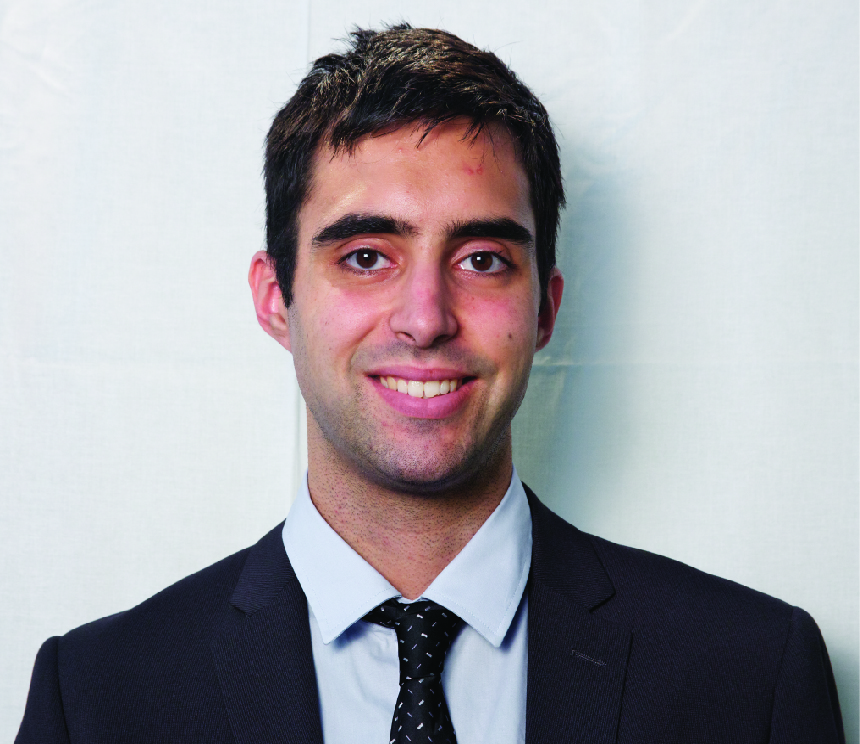
\includegraphics[trim= 320 130 460 210,clip,width=0.2\linewidth]{Foto_Smart.jpg}  %trimming relative to image size!
    %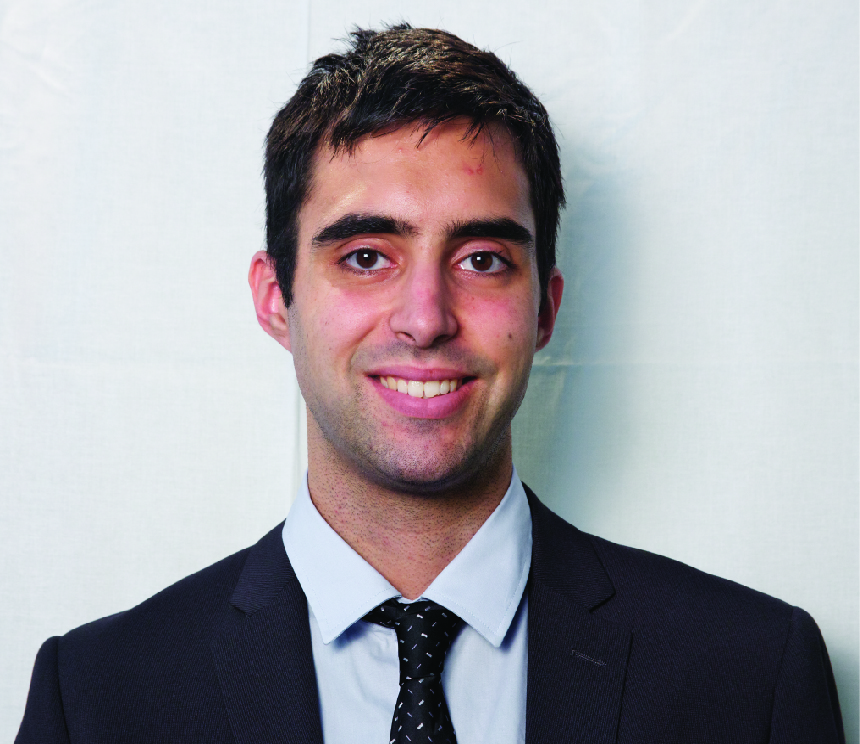
\includegraphics[width=0.2\linewidth]{Foto_Smart.jpg}
%\end{flushright}
%\end{figure}

%---------------------------------------------------------------------------------------
%  QR CODE (optional)
%----------------------------------------------------------------------------------------
%\vspace{-136pt}
%\hspace{0.75\linewidth}
%
\includegraphics[width=103pt]{qrcode}
%\normalsize
%\vspace{88pt}

%---------------------------------------------------------------------------------------
%  META SECTION
%----------------------------------------------------------------------------------------

%\vspace{-114pt}

%\metasection{Status:}{M.Sc. Digital Media, IT Consultant at We4IT Bremen}
%\metasection{Fields:}{Project Management, Software Development, Scrum, Usability}
%\metasection{Prefers:}{JS, Java, XPages, Flex / AIR, Processing, Git, Eclipse}
%\metasection{Activities:}{Global Game Jam, Sound Engineering, Blender, Martial Arts}

%\vspace{6pt}

%---------------------------------------------------------------------------------------
%  SUMMARAY (optional)
%----------------------------------------------------------------------------------------

%\cvsection{Summary}\\
%Digital media graduate with four years project experience in the field of technology based assessment. Specialized in development of test-scenario engines and innovative, rich media item formats. Master studies focused on teams from different disciplines and cultural backgrounds on solutions for complex problems.  Prior knowledge has been collected in he field of usability / accessibility during bachelor studies.\\

%============================================================================%
%
%  CV SECTIONS AND EVENTS (MAIN CONTENT)
%
%============================================================================%
%---------------------------------------------------------------------------------------
%  EXPERIENCE
%----------------------------------------------------------------------------------------
\cvsection{Exp\'eriences professionnelles}
\cvevent{07/`22-}%
        {Ing\'enieur-chercheur}%
        {ONERA, Ch\^atillon}%
        {Sch\'emas et m\'ethodes num\'eriques. Gestion de \href{\NextSimlink}{projets de recherche}. Encadrement de \href{\articleJeanlink}{stages} et th\`eses. IA pour la CFD}%
        {D\'eveloppement (CODA, \CoMMAhref). Calcul parall\`ele. Gestion d'installations sur calculateurs}

%
\cvevent{01/`21-04/`22}%
        {Charg\'e de recherche (PostDoc)}%
        {CEREA - \'Ecole des Ponts ParisTech}%
        {\SciencesJOhref{}, la physique des sports. Tir \`a l'arc: support et am\'elioration de performance}%
        {Simulations CFD de vol de fl\`eche, analyse statistique, reconnaissance d'image}

%
\cvevent{09/'16-02/'17}%
        {Stage de recherche, 6 mois}%
        {EDF R\&D, Chatou}%
        {D\'eveloppement et analyse num\'erique de la m\'ethode \href{\tesilink}{\emph{Hybrid High-Order} pour la diffusion} anisotrope en 3D}%
        {Int\'egration dans le code industriel \cs{} (\texttt{C}); parall\'elisation \`a l'aide de OpenMP}

%\textcolor{softcol}{\hrule}

%
\cvevent{03-08/2015}%
        {Stage de recherche, 5 mois}%
        {US ESI R\&D, San Diego}%
        {Premiers d\'eveloppements pour une nouvelle m\'ethode de calcul rapide de la r\'eponse vibro-acoustique d'un syst\`eme}%
        {Validation avec simulations (MATLAB)}

%\textcolor{softcol}{\hrule}

%
%\cvevent{08/2014}%
        %{Stage d'\'et\'e, 1 mois}%
        %{VTB Bank, Irkutsk}%
        %{Groupe de contr\^ole des devises \'etrang\`eres}%
        %{Aide \`a la pr\'eparation et \`a la validation finale de contrats internationaux; gestion d'archives}


\vspace{8pt}


%---------------------------------------------------------------------------------------
%  EDUCATION SECTION
%--------------------------------------------------------------------------------------
\cvsection{Formation}

\cvevent{2017 - 2020}%
        {Doctorat en Math\'ematiques Appliqu\'ees}%
        {\'Ecole des Ponts ParisTech et INRIA EDF R\&D}%
        {Th\`ese CIFRE: \href{\PhDlink}{Sch\'emas \emph{Compatible Discrete Operator}} pour les \'equations de Navier–Stokes d’un fluide incompressible en r\'egime instationnaire. Directeur: Ern Alexandre (ENPC, INRIA); Encadrant industriel: Bonelle J\'er\^ome (EDF R\&D)}%
        {\href{\articlelink}{Article dans journal avec comit\'e de relecture}: \article{}}

%\cvevent{2015 - 2017}%
        %{Master 2 en Ing\'enierie}%
        %{Politecnico di Milano}%
        %{\href{https://www.politesi.polimi.it/handle/10589/133692}{\emph{Laurea Magistrale}} en Ing\'enierie Math\'ematique, sp\'ecialisation: Math\'ematiques Appliqu\'ees \& Sciences Informatiques}%
        %{Note: 110/110 avec mention}

%\textcolor{softcol}{\hrule}

%
\cvevent{2013 - 2017}%
        {Cycle de l'Ing\'enieur \textit{Polytechnicien}}%
        {\'Ecole polytechnique}%
        {Dipl\^ome d'ing\'enieur de l'\'Ecole polytechnique et Master}%
        {Programme d'Approfondissement : Math\'ematiques Appliqu\'ees - EDP et analyse num\'erique}

%\textcolor{softcol}{\hrule}

%
\cvevent{2010 - 2017}%
        {Licence et Master en Ing\'enierie}%
        {Politecnico di Milano}%
        {\emph{Laurea Triennale} et \emph{Laurea Magistrale} en Ing\'enierie Math\'ematique. Sp\'ecialisation: Math\'ematiques Appliqu\'ees \& Sciences de l'information}%
        {Note: 110/110 avec mention (licence et master). \'Elu meilleur \'el\`eve de premi\`ere ann\'ee apr\`es r\'esultats du test d'admission et des examens du premier semestre (2010)}

\vspace{8pt}

\begin{minipage}{.48\linewidth}
\begin{flushleft}
\cvsubsection{Comp\'etences informatiques}
\vspace{4pt}
\begin{tabular*}{1\linewidth}{l l}
&     \larrow{bgcol} \textbf{Connaissance approfondie}: \texttt{C}/\texttt{C++}, OpenMP, MPI,\\[3pt]
&       \TeXtipshref{}, Unix, \texttt{python}, Git/SVN, shell script, spack,\\[3pt]
&       \CShref{}, Office\\[3pt]
&     \larrow{bgcol} \textbf{Notions de base}: MATLAB, Fortran, OpenCV, \texttt{R},\\[3pt]
&       Rust, SALOME%FreeFem\texttt{++}, Java
\end{tabular*}
\end{flushleft}
\end{minipage}
\hfill
\begin{minipage}{.48\linewidth}
\begin{flushright}
\cvsubsection{Activit\'es extra-professionnelles}
\vspace{6pt}
\begin{tabular*}{1\linewidth}{l l}
&     \larrow{bgcol} Invitation au Google FooBar Challenge\\[3pt]
&     \larrow{bgcol} Responsable d'un foyer \'etudiant ('15)\\[3pt]
&     \larrow{bgcol} Tr\'esorier de l'\AIMhref{en} ('16)\\[3pt]
&     \larrow{bgcol} Doctorant r\'ef\'erent pour EDF-MFEE ('18-'20)\\[3pt]
&     \larrow{bgcol} Running (marathon de Paris '19, '24)\\[3pt]
\end{tabular*}
\end{flushright}
\end{minipage}

\vspace{4pt}

\begin{minipage}{.48\linewidth}
\begin{flushleft}
\cvsubsection{Langues}
\vspace{4pt}
\begin{tabular*}{1\linewidth}{l l l}
&     \larrow{bgcol} \textbf{Italien}:          &Langue maternelle\\[3pt]
&     \larrow{bgcol} \textbf{Français}:         &Courant, certificat TCF, C1\\[3pt]
&     \larrow{bgcol} \textbf{Anglais}:          &Courant, certificat FCE, B2\\[3pt]
&     \larrow{bgcol} \textbf{Allemand, Russe}:  &Notions\\[3pt]
\end{tabular*}
\end{flushleft}
\end{minipage}
\hfill
\begin{minipage}{.48\linewidth}
\begin{flushright}
\cvsubsection{Centres d'int\'er\^et et B\'en\'evolat}
\vspace{4pt}
\begin{tabular*}{1\linewidth}{l l}
&     \larrow{bgcol} Camps d'\'et\'e (Kenya '10, '11; Rwanda '17)\\[3pt]
&     \larrow{bgcol} Membre de l'association Smileland, qui fournit\\[3pt]
&        de l'aide humanitaire au Congo (`15-`22)\\[3pt]
&     \larrow{bgcol} Professeur d'italien pour les r\'efugi\'es ('15)\\[3pt]
\end{tabular*}
\end{flushright}
\end{minipage}




%-------------------------------------------------------------------------------------------------
%  ARTIFICIAL FOOTER (fancy footer cannot exceed linewidth)
%--------------------------------------------------------------------------------------------------

\null
\vspace*{\fill}
%\hspace{-0.25\linewidth}\colorbox{bgcol}{\makebox[1.5\linewidth][c]{\mystrut \small \textcolor{white}{www.jankuester.com} $\cdot$ \textcolor{white}{github.com/jankapunkt}}}




%============================================================================%
%
%
%
%  DOCUMENT END
%
%
%
%============================================================================%
\end{document}
